
\chapter{枝刈りによる探索空間の削減}
\label{chap:reduce-by-prune}
枝刈りによって探索空間を削減する.
本稿では,直径の下界を計算し,定理\ref{theorem:gmg-geometric-property}
の条件\ref{gmg-geom-b}を満足するか求めることで実現する.

\section{直径の下界の計算}
\label{sect:distance-lower-bound}
直径の下界を計算する方法を与える.まず,次のグラフを定義する.
\begin{definition}
  探索途中のグラフ$G$が与えられ,$i$番目の辺$f_i\in F$の追加判定および追加が
  行われたとする.$G$の辺と追加が未決定の辺すべて($\{f_j\}_{j>i}\subseteq F$)
  を合わせたグラフを\textbf{最大グラフ}と定義する.
  このとき,最大グラフのもとになったグラフを\textbf{最小グラフ}と呼ぶ.
\end{definition}
\begin{example}
  図\ref{fig:min-max-graph}に例を示す.最小グラフの破線部分は追加の
  判定が行われていない辺を表す.最大グラフは,最小グラフの追加未決定の辺を
  すべて追加したグラフとなっている.
\end{example}
\begin{figure}
  \centering
  \subfloat[最小グラフ]{
    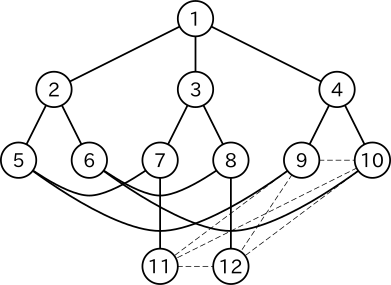
\includegraphics[width=.4\linewidth]
                    {min-graph-example.pdf}
  }\hfill
  \subfloat[最大グラフ]{
    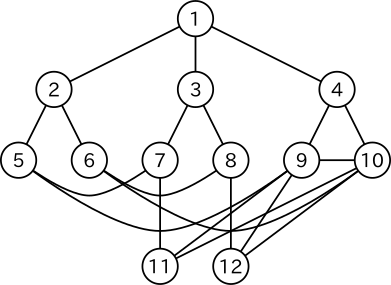
\includegraphics[width=.4\linewidth]
                    {max-graph-example.pdf}
  }
  \caption{最小グラフと最大グラフの例}
  \label{fig:min-max-graph}
\end{figure}

直径の下界は,最大グラフの直径を計算すればよい.もし直径の下界が
定理\ref{theorem:gmg-geometric-property}の条件\ref{gmg-geom-b}を
満たさない場合,それはどのように辺を追加しても条件を満たさないので,
その場で探索を打ちきることができる.

\section{頂点間距離の高速な更新法}
\label{sect:faster-min-max}
第\ref{chap:basic-algorithm}章において,グラフが枝刈りの対象となるかを
判定するには,追加する辺の頂点間距離と直径の下界を求める必要があることを述べた.
本節では,これらの値を高速に計算するため,辺の追加と削除に対して,頂点間距離と
直径の下界を更新するアルゴリズムを与える.
探索空間の削減にはつながらないが,計算量が削減され,実行時間の短縮が期待できる.
また,この方法は辺の追加と削除に対する媒介中心性の高速な計算法への応用が期待できる.

グラフ$G=(V,E),V=\{1,\ldots n\}$のすべての頂点の組$(s,t)$の距離$d(s,t)$と
距離が$d(s,t)$となる最短経路の数$\sigma(s,t)$が与えられているとする.
まず,追加と削除に共通するいくつかの補題を示す.
\begin{lemma-without-proof}[Brandes]
  foo
\end{lemma-without-proof}
\begin{lemma}[難波ら]
  bar
\end{lemma}
\begin{proof}
  bar
\end{proof}
\begin{lemma-without-proof}[Brandes]
  foo
\end{lemma-without-proof}
\begin{lemma}[難波ら]
  bar
\end{lemma}
\begin{proof}
  bar
\end{proof}

次の定理は,ある2頂点の最短経路の数と,その経路に含まれる短い最短経路の数との
関係を示す.
\begin{theorem}
  \label{theorem:number-of-paths}
  $d(s,t)=d(s,v)+d(v,t)$である$v\in V$(ただし$v\neq s,v\neq t$)について,
  \begin{equation}
    \label{eq:number-of-paths}
    \sigma(s,t)=\left(
    \sum_{v}\sigma(s,v)\sigma(v,t)\right) / (d(s,t)-1)
  \end{equation}
  が成り立つ.
\end{theorem}
\begin{proof}
  $s$と$t$の間の一般的な経路を図\ref{fig:proof-number-of-paths}に示す.
  \begin{figure}
    \centering
    \def\svgwidth{.5\columnwidth}
    \input{proof-number-of-paths.pdf_tex}
    \caption{$s$と$t$の一般的な最短経路}
    \label{fig:proof-number-of-paths}
  \end{figure}
  $s$からの距離が一定の頂点を並べて,一つの層とする.$d(s,v)=k$なる頂点
  $v$の集合を,第$k$層と定義し,$L_k$と表す.
  $L_k$に属する頂点の数を$n_k$,$l$番目の頂点を$v_{kl}$と表す.
  ここで,すべての層に属する頂点$v$は,隣接する層以外の層に属する頂点$w$と
  隣接しないことに注意する.もしそのような頂点が存在すると,最短経路長が
  変化する.式\ref{eq:number-of-paths}の両辺に$d(s,t)-1$を掛けて,
  \begin{equation}
    \sigma(s,t)(d(s,t)-1)=\sum_{v}\sigma(s,v)\sigma(v,t)
    \label{eq:number-of-paths1}
  \end{equation}
  となる.式\ref{eq:number-of-paths1}の右辺を,
  図\ref{fig:proof-number-of-paths}にならって変形して,
  \begin{equation}
    \sum_{v}\sigma(s,v)\sigma(v,t)=
    \sum_{k=1}^m\sum_{l=1}^{n_k}\sigma(s,v_{kl})\sigma(v_{kl},t)
    \label{eq:number-of-paths2}
  \end{equation}
  とする.二つの頂点$v$と$w$について,
  \begin{align*}
    a(v,w)=
    \begin{cases}
      1 & vとwが隣接しているとき \\
      0 & vとwが隣接していないとき
    \end{cases}
  \end{align*}
  と定義する.
  各々の$\sigma(s,v_{kl})\sigma(v_{kl},t)$について議論する.
  定義に沿って式を変形すると,
  \begin{align}
    &\sigma(s,v_{kl})\sigma(v_{kl},t)\nonumber\\
    =&\left(\sum_{v'\in L_{k-1}}\sigma(s,v')a(v',v_{kl})\right)
    \left(\sum_{v'\in L_{k+1}}\sigma(v_{kl},v')a(v',t)\right)
    \nonumber\\
    =&\left(\sum_{v''\in L_{k-2}}\sum_{v'\in L_{k-1}}
    \sigma(s,v'')a(v'',v')a(v',v_{kl})\right)
    \left(\sum_{v'\in L_{k+1}}\sum_{v''\in L_{k+2}}
    a(v_{kl},v')a(v',v'')\sigma(v'',t)\right)
    \nonumber\\
    &\vdots\nonumber\\
    =&\left(\sum_{(v_1,\ldots,v_{k-1})\in L_1\times\cdots\times L_{k-1}}
    a(s,v_1)\cdots a(v_{k-1},v_{kl})\right)
    \left(\sum_{(v_{k+1},\ldots,v_m)\in L_{k+1}\times\cdots\times L_m}
    a(v_{kl},v_{k+1})\cdots a(v_m,v_t)\right)\nonumber\\
    =&\sum_{
      (v_1,\ldots,v_{k-1},v_{k+1},\ldots,v_m)\in
      L_1\times\cdots\times L_{k-1}\times L_{k+1}\times\cdots\times L_m
    }
    a(s,v_1)\cdots a(v_{k-1},v_{kl})a(v_{kl},v_{k+1})\cdots a(v_m,t)
    \label{eq:number-of-paths3}
  \end{align}
  となる.式\ref{eq:number-of-paths3}を式\ref{eq:number-of-paths2}に
  代入すると,
  \begin{align}
    &\sum_{k=1}^m\sum_{l=1}^{n_k}\sigma(s,v_{kl})\sigma(v_{kl},t)\nonumber\\
    =&\sum_{k=1}^m\sum_{l=1}^{n_k}\sum_{
      (v_1,\ldots,v_{k-1},v_{k+1},\ldots,v_m)\in
      L_1\times\cdots\times L_{k-1}\times L_{k+1}\times\cdots\times L_m
    }
    a(s,v_1)\cdots a(v_{k-1},v_{kl})a(v_{kl},v_{k+1})\cdots a(v_m,t)\nonumber\\
    =&\sum_{k=1}^m\sum_{(v_1,\ldots,v_m)\in L_1\times\cdots\times L_m}
    a(s,v_1)\cdots a(v_m,t)\nonumber\\
    =&m\left(\sum_{(v_1,\ldots,v_m)\in L_1\times\cdots\times L_m}
    a(s,v_1)\cdots a(v_m,t)\right)
    \label{eq:number-of-paths4}
  \end{align}
  とできる.式\ref{eq:number-of-paths4}の総和の対象が$1$となるのは,
  $a(s,v_1),\ldots,a(v_m,t)$のすべてが$1$のとき,
  すなわち,$s$と$t$の最短経路となっているときである.
  従って,総和の値は$s$と$t$の最短経路の数を一致し,
  式\ref{eq:number-of-paths4}は$m\sigma(s,t)$と等しい.
\end{proof}

\subsection{辺の追加に対する頂点間距離の更新}
\label{subsect:update-path-length}
$G$に辺$e=\{\alpha,\beta\}\notin E(G)$を追加したた後の頂点間距離$d'(s,t)$と
最短経路数$\sigma'(s,t)$を求める.
一般性を失うことなく,$s<t,\,d(s,\alpha)\leq d(s,\beta)$とできる.

\subsection{辺の削除に対する頂点間距離の更新}
\label{subsect:update-lower-bound-of-diameter}
$G$から辺$e=\{\alpha,\beta\}\in E(G)$を削除した後の頂点間距離$d'(s,t)$と
最短経路数$\sigma'(s,t)$を求める.
一般性を失うことなく,$s<t,\,d(s,\alpha)\leq d(s,\beta)$とできる.

まず,辺の削除に影響される頂点の組$(s,t)$を考える.そのような頂点の組は,
最短経路に辺$e$が含まれている.すなわち,$d(s,t) = d(s,\alpha)+d(\beta,t)+1$
が成り立つことである.そのような$(s,t)$に対して,辺$e$を含まない最短経路の数は,
$\overline{\sigma(s,t)}=\sigma(s,t)-\sigma(s,\alpha)\sigma(\beta,t)$で
与えられる.$\overline{\sigma(s,t)}=0$ならば,$s$と$t$の最短経路はすべて
$e$を含むので,距離を更新する必要がある.そのような$(s,t)$の列を
$P=\{(s_i,t_i)\}$で表す.
逆に,$\overline{\sigma(s,t)}>0$ならば,$s$と$t$の最短経路に$e$を含まない
ものが存在し,距離の更新は行われず,最短経路の数が
$\sigma(s,\alpha)\sigma(\beta,t)$だけ減少する.つまり,
$d(s,t)<d(s,\alpha)+d(\beta,t)+1$または$\overline{\sigma(s,t)}>0$となる
$(s,t)$に対して,
\begin{align*}
  d'(s,t) &\gets d(s,t) \\
  \sigma'(s,t) &\gets
  \begin{cases}
    \sigma(s,t) & d(s,t) < d(s,\alpha) + d(\beta,t) + 1 \\
    \overline{\sigma(s,t)} & d(s,t) = d(s,\alpha) + d(\beta,t) + 1
  \end{cases}
\end{align*}
が成り立つ.

先述のとおり,そのような頂点の組は,
$d(s,t)=d(s,\alpha)+d(\beta,t)+1$かつ$\overline{\sigma(s,t)}=0$
となる$(s,t)$である.まず,距離$d'(s,t)$から求める.すべての頂点$v$について,
$d(s,v)+d(v,t)$の最小値を求める.ただし,$s$と$v$の最短経路もしくは$v$と$t$の
最短経路に$e$が含まれないものを選ぶ.経路が$e$を含むかどうかの判定は先述のとおり.
よって,更新後の距離$d'(s,t)$は,
\begin{align*}
  d'(s,t) = \min_{v\in V}(d(s,v)+d(v,t)\:|\:
  &(d(s,v)<d(s,\alpha)+d(\beta,v)+1\,または\,\overline{\sigma(s,v)}>0),\\
  &(d(v,t)<d(v,\alpha)+d(\beta,t)+1\,または\,\overline{\sigma(v,t)}>0))
\end{align*}
で与えられる.

次に,距離の更新が行われる組$(s,t)$の$\sigma'(s,t)$について議論する.
まず,準備のため次を示す.
\begin{collary}
  $\sigma'(s,t)$を再計算するには,すべての$d'(s,t)>d'(u,v)$の$\sigma'(u,v)$
  を先に計算しなければならない.
\end{collary}
\begin{proof}
  定理\ref{theorem:number-of-paths}の式\ref{eq:number-of-paths2}を見ると,
  $s$と$t$の最短経路の中に$d'(s,t)>d'(u,v)$なる$u$と$v$の最短経路が含まれ,
  そのような$u,v$に対する$\sigma'(u,v)$が含まれる.
\end{proof}

$P$を$d'(s,t)$の昇順に並べ替え,$P'=\{(s'_i,t'_i)\}$を得る.
最後に,定理\ref{theorem:number-of-paths}の式を用いて,
$\sigma'(u,v)$を求める.

最後に,アルゴリズムをアルゴリズム\ref{algo:update-distance-on-remove}に示す.
\begin{algorithm}
  \caption{辺$\{\alpha,\beta\}$が削除されたときの$d'(s,t)$と$\sigma'(s,t)$の
  計算}\label{algo:update-distance-on-remove}
  \begin{algorithmic}[1]
    \Require $G=(V,E),\,d(s,t),\,\sigma(s,t)$
    \Ensure $d'(s,t),\,\sigma'(s,t)$
    \Procedure{Free From Delete}{$s,t,\alpha,\beta$}
    \State $\{\alpha,\beta\}$のうち,$s$に近い方を$\alpha$,
    それ以外を$\beta$とする.
    \State \textbf{return} $d(s,t)<d(s,\alpha)+d(\beta,t)$もしくは
    $\sigma(s,t)>\sigma(s,\alpha)\sigma(\beta,t)$
    \EndProcedure
    \Procedure{Update Distance on Remove}{$\alpha,\beta$}
    \State $P\gets\varnothing$
    \ForAll{$(s,t)\in V\times V$}
    \Comment{更新の対象となる頂点組$(s,t)$を求める}
    \If{$d(s,t)<d(s,\alpha)+d(\beta,t)+1$}
    \State $d'(s,t)\gets d(s,t),\,\sigma'(s,t)\gets\sigma(s,t)$
    \ElsIf{$\sigma(s,t)>\sigma(s,\alpha)\sigma(\beta,t)$}
    \State $d'(s,t)\gets d(s,t),\,\sigma'(s,t)\gets\sigma(s,t)
    -\sigma(s,\alpha)\sigma(\beta,t)$
    \Else\Comment{距離更新が必要}
    \State $d'(s,t)\gets\infty,\,\sigma'(s,t)\gets0,\,P\gets P\cup\{(s,t)\}$
    \EndIf
    \EndFor
    \ForAll{$(s,t)\in P$}\Comment{距離を更新}
    \State $d_{\min}\gets\infty$
    \ForAll{$v\in V$}
    \If{\Call{Free From Delete}{$s,v,\alpha,\beta$}かつ
      \Call{Free From Delete}{$v,t,\alpha,\beta$}}
    \If{$d(s,v)+d(v,t)<d_{\min}$}
    \State $d_{\min}\gets d(s,v)+d(v,t)$
    \EndIf
    \EndIf
    \EndFor
    \State $d'(s,t)\gets d_{\min}$
    \EndFor
    \State $P$を$d'(s,t)$の昇順にソートし,$P'=\{(s'_i,t'_i)\}$を得る
    \ForAll{$i=\{1,\ldots|P'|\}$}\Comment{最短経路数を更新}
    \State $\sigma_{\mathrm{sum}}\gets0$
    \ForAll{$v\in V$}
    \If{$d'(s'_i,t'_i)=d'(s'_i,v)+d'(v,t'_i)$}
    \State $\sigma_{\mathrm{sum}}\gets
    \sigma_{\mathrm{sum}}+\sigma'(s'_i,v)\sigma'(v,t'_i)$
    \EndIf
    \EndFor
    \State $\sigma'(s_i,t_i)\gets\sigma_{\mathrm{sum}}/(d'(s_i,t_i)-1)$
    \EndFor
    \EndProcedure
  \end{algorithmic}
\end{algorithm}

\section{実験}

\section{結果}

